% -----------------------------------------------
% Vlastní text práce (kapitoly práce)
% -----------------------------------------------

% -----------------------------------------------
\chapter{Calibration UV optical source}
% -----------------------------------------------
 \label{chap4}
As was mentioned before, the calibration UV optical source is an essential instrument to perform calibrations. Its main purpose is to deliver stable intensity which does not vary over time or due to the changes in outer conditions.
\par
In case of FAST the process of calibration requires low-intensity UV light to be delivered in microsecond square pulses. This is because FAST is a low-intensity detector and its PMTs may be easily saturated.

% -----------------------------------------------
\section{UV source}
% -----------------------------------------------
For the calibration purposes was developed a prototype of pulse UV source based on the current-driven LEDs inspired by the Karlsruhe Institute of Technology (KIT) concept. The active parts - LED drive circuit and 3 LEDs are situated in temperature stabilized head. 
\par
The source is driven by STM32 board, which allows us to set parameters - LED current, PWM duty and frequency.
 


 \begin{figure}[H]
 \centering
 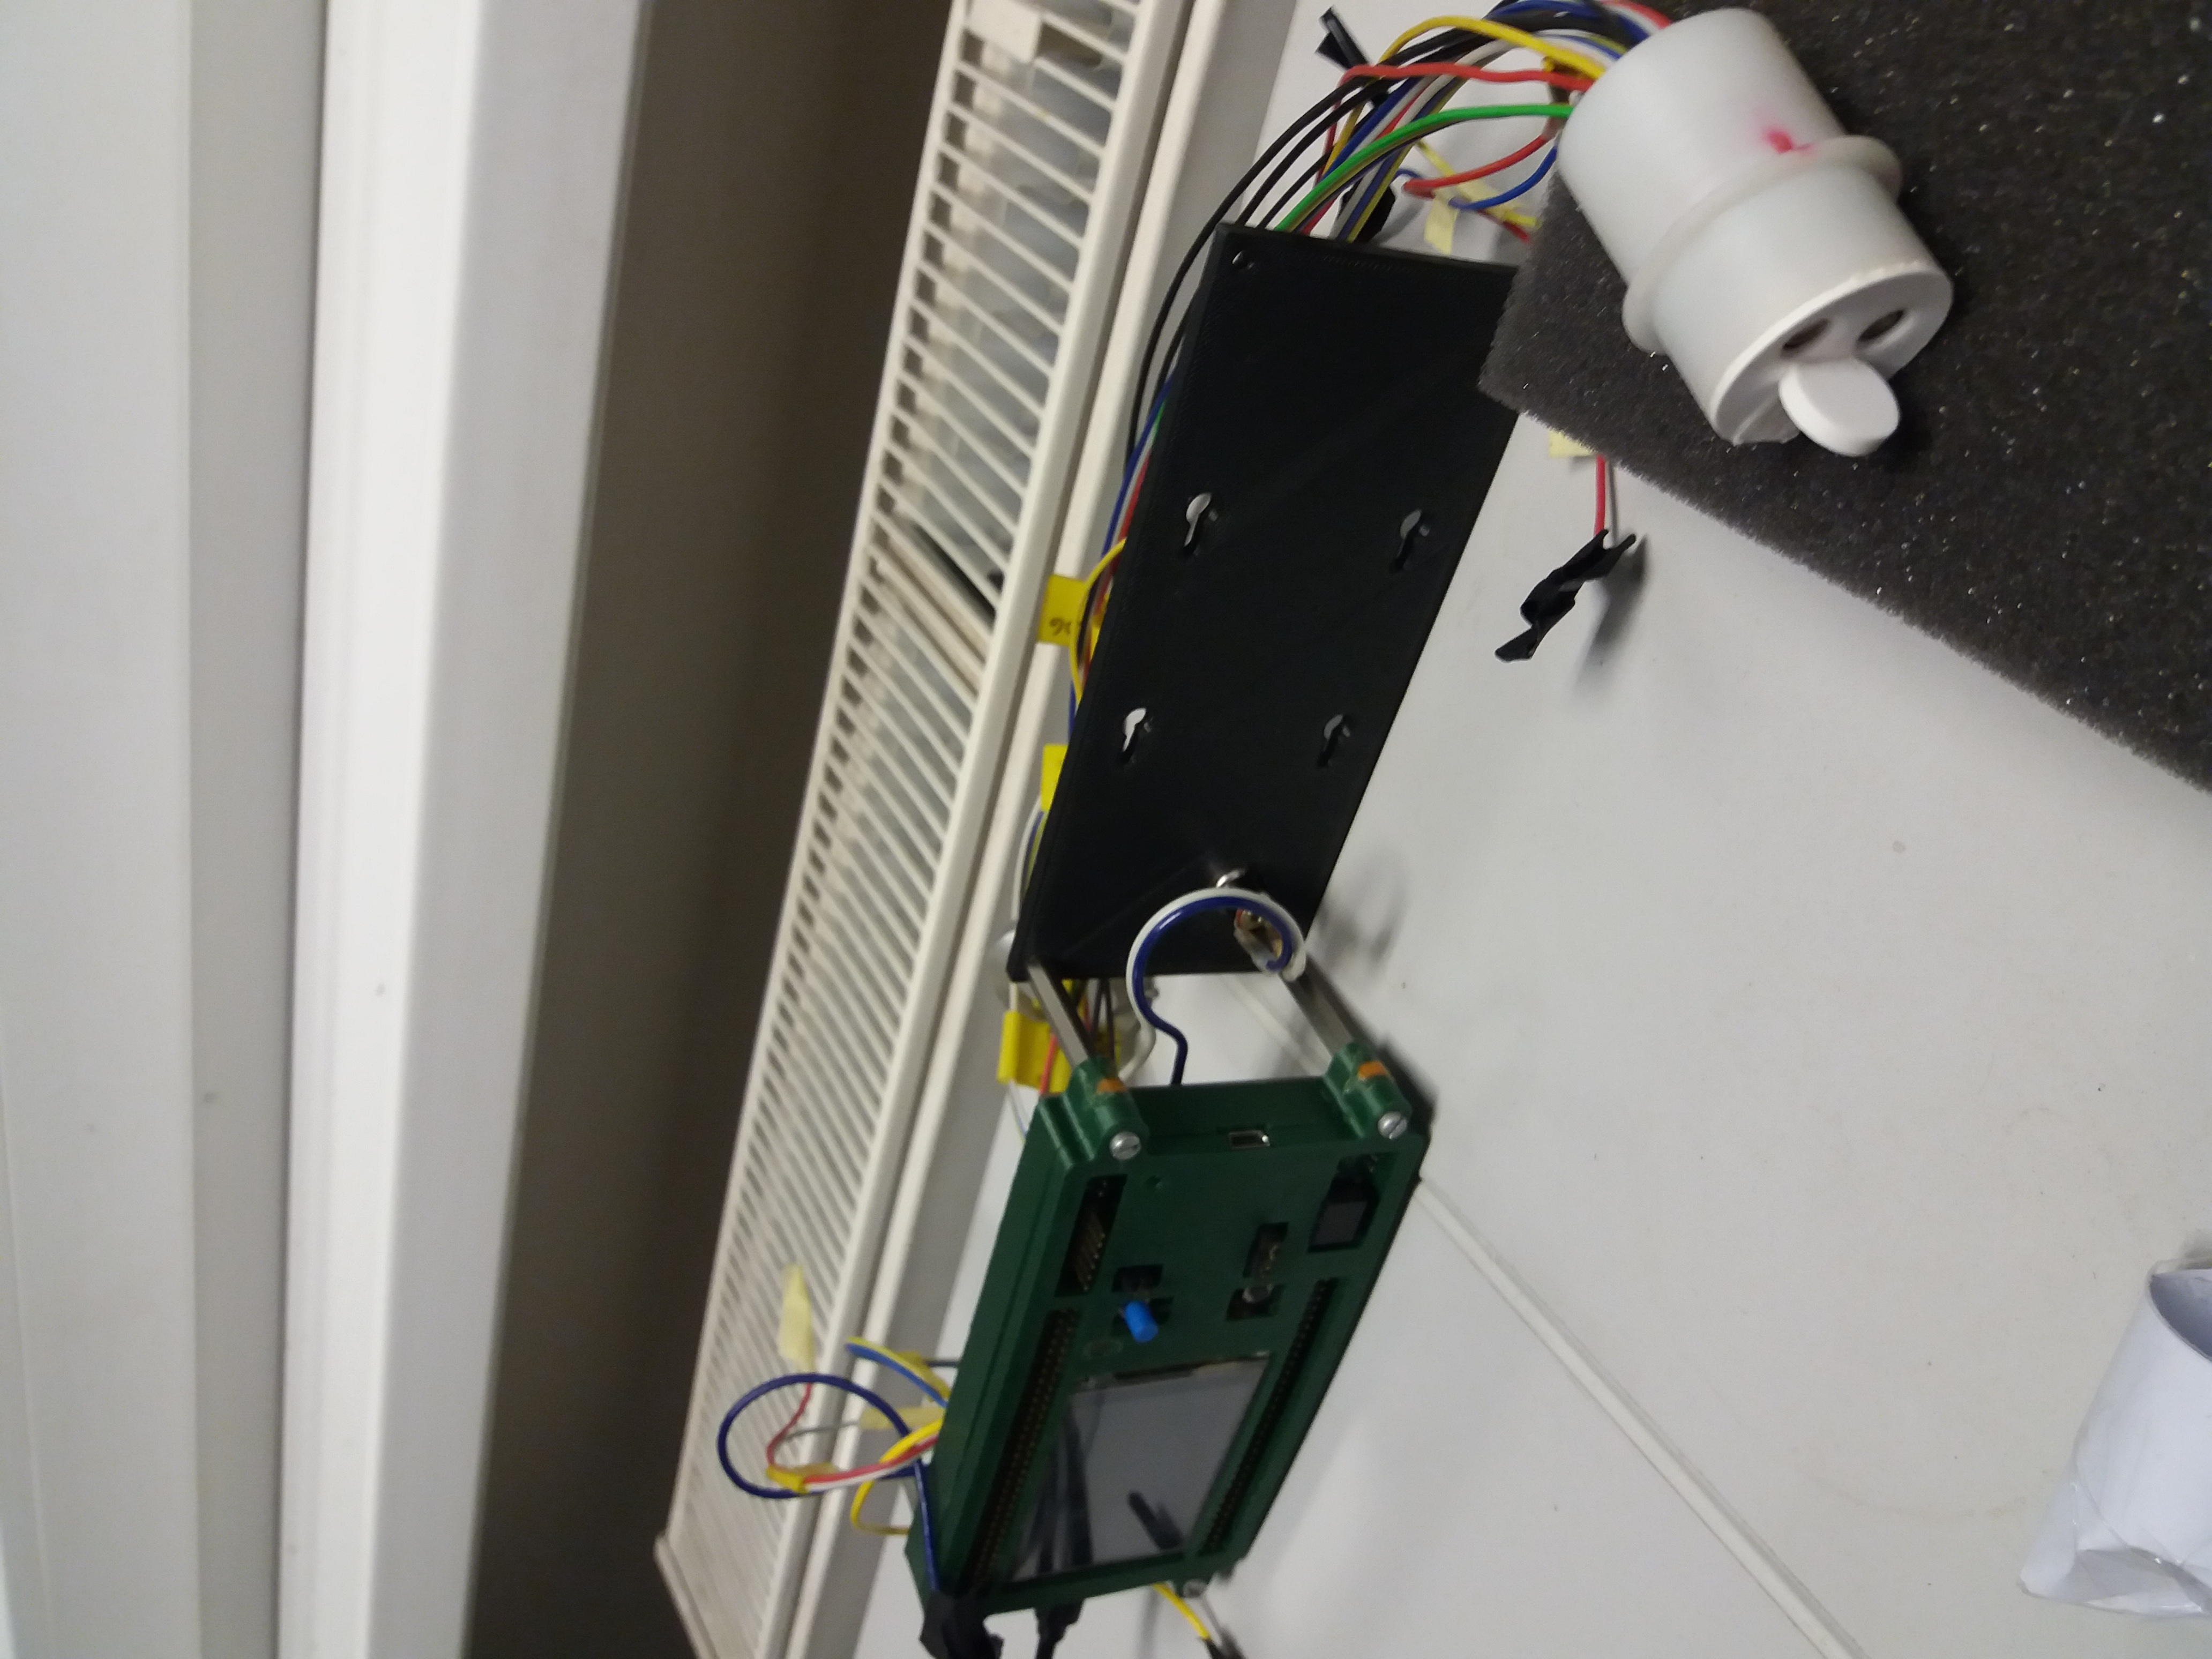
\includegraphics[scale=0.09, angle = 270, origin = c]{./pictures/KarlsRuhe}
 \caption{UV source conctructed by Vladimír Urbášek from SLO.}
 \label{UVsource}
\end{figure}

 \begin{figure}[H]
 \centering
 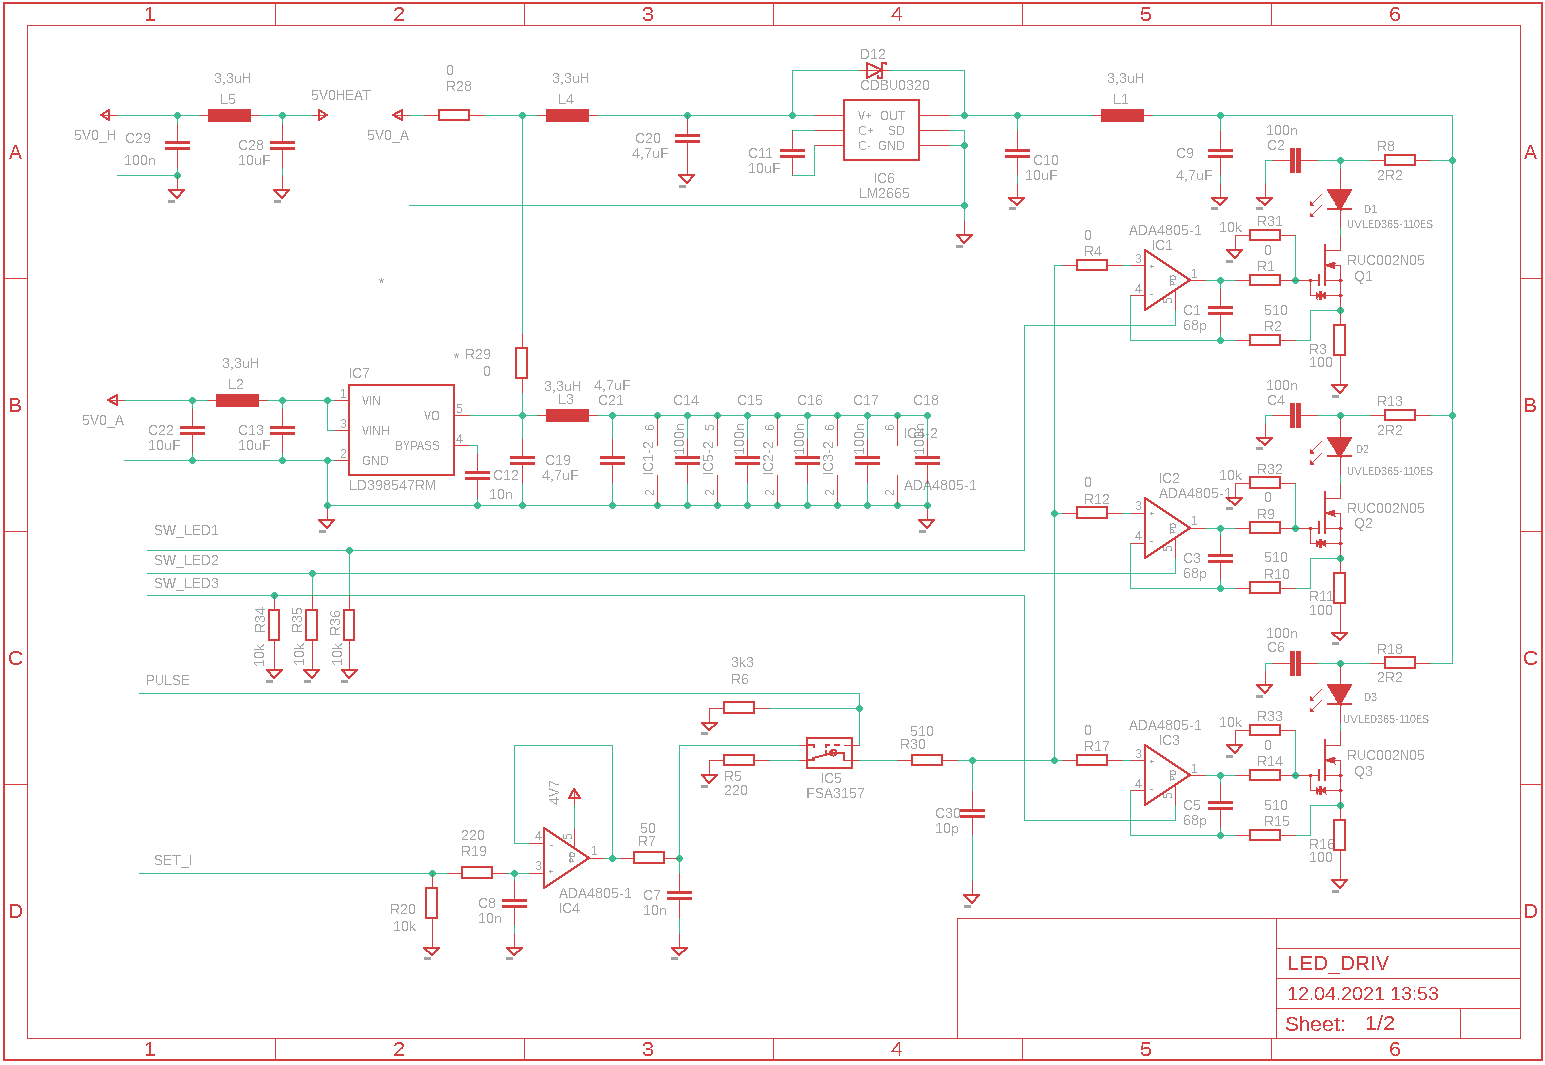
\includegraphics[scale=0.5, angle = 0, origin = c]{./pictures/OrigScheme.png}
 \caption{UV source schematic. On the right side we can see the pulse current drivers for three LEDs with the feedback Op amps as the main component.}
 \label{UVsource}
\end{figure}


Our main task was to test this UV source's long-time stability and develop possible fixes and upgrades.

% -----------------------------------------------

\section{Testing and measurement of UV source}
% -----------------------------------------------
For calibration UV source, the long-time stability of optical power and pulse geometry is very important. Because there was no specialized apparatus for this measurement, we had to make our own. For these measurements, we use UV source with LED current $I_{\textrm{d}}$ = 2.5 mA, 50$\%$ duty cycle and frequency $f = 50$ kHz. 
\subsection{Measuring apparatus}
For measuring the optical power we use PM16 power meter (PM) and for determining the pulse geometry we use XP2262 PMT with signal output connected to 2-channel PicoScope 2205A MSO usb oscilloscope. XP2262 PMT is held on $U \approx -680$ V by HV voltage source. The PMT's gain may drift over time, but we use PMT mainly for geometry analysis and measurement of absolute optical power is left to PM16.
\par
We also use DS18B20 thermometer for PMT temperature monitoring and keysight 34461a multimeter for readout voltages.

\par
The PMT, power meter and the optical head of UV source are mounted in the IS's ports. The IS stops the unwanted external light and distributes the optical power to PMT and power meter. 
\par
The entire apparatus is driven by Raspberry Pi (RPi). The RPi takes care of data acquisition and can be used to set the parameters of the UV source. It can be easily accessed over internet for data download or for user to control the experiment.
\par
Osciloscope's readout was programmed in C language according to its programmer's manual \cite{PicoScope}. It is capable of 2ns sampling which is enough to capture rising edges of the pulses. The RPi sets basic parameters (DC coupling, range etc.) and then activates oscilloscope's trigger (rising edge). After sampling, RPi receives all samples from oscilloscope's memory.
\par
The multimeter is controlled by VISA commands using python USBTMC library. For thermometer we use RPi's 1-Wire.
\par
Main component (IS,PW, PMT with HV source, UV source) are situated in protection box to prevent unwanted manipulations and touching the HV parts.The apparatus can be seen on fig. \ref{aparature1} and \ref{aparature2}.

\begin{figure}[H]
 \centering
 \includegraphics[width=150mm]{./pictures/aprature1b}
 \caption{Measuring apparatus.}
 \label{aparature1}
\end{figure}

\begin{figure}[H]
 \centering
 \includegraphics[scale = 0.09]{./pictures/aparature2b}
 \caption{PMT mounting and HV source.}
 \label{aparature2}
\end{figure}


\subsection{Data acquisition and analysis}
All the data are taken in specified interval (15 or 30 minutes). Two files are produced - osciloscope waveform file and a file with 30 samples of power meter, multimeter and a thermometer readings. From these 30 samples we calculate average and error. Most of data analysis we perform is done by C/C++ Root framework.
\par
The data from oscilloscope contains the square pulses with noise (fig. \ref{pulse}). From them we need to extract the information of pulses height, slope and time of the rising edge.

 \begin{figure}[H]
 \centering
 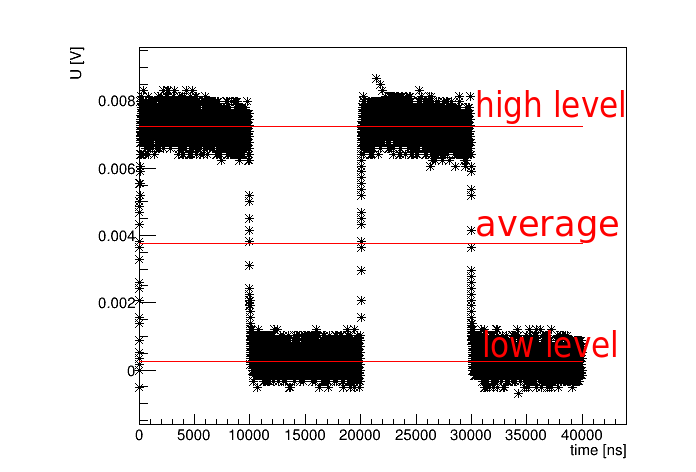
\includegraphics[scale=0.65]{./pictures/PMTPulse}
 \caption{Determining the basic pulse properties - average, low and high levels of signal.}
 \label{pulse}
\end{figure}

To determine the pulse height, we need to calculate the average value from all the samples at first. Then, we split the samples into two subgroups according to fact, whether they are higher or lower than the average. These subgroups are converted to histograms with fixed binning (around 5000 bins). These histograms are then fitted by gaussian. The means of these two fits determine two levels of the pulse - high ($U_\textrm{h}$) and low ($U_\textrm{l}$). The fig. \ref{pulse} shows the real pulse with levels determined by this method. The height of pulse is then simply calculated by subtracting two levels: $U_\textrm{H} = U_\textrm{h} - U_\textrm{l}$.

\par
The properties of the rising edge can be specified by two parameters, which we are able to extract from our data - time and the slope of the rising edge. We are able to calculate both of them if we identify the samples of the rising edge. These samples' values should be between 20 $\%$ and 80 $\%$ of the $U_{H}$. First, we need to detect the rising edge in waveform data sequence. However, the signal is very noisy and this can not be simply done by detecting the exceeding of the 10 $\%$ of the $U_{H}$ .To achieve that, we cycle through the waveform until we meet two conditions - the value is higher than average (and lesser than $80 \%$) and the derivative is positive. Due to the noise, the derivative could not be calculated from two or three points, thus we use Savitzky–Golay polynomial's derivative at chosen point: $y' = \frac{1}{12h}(y_{i-2} -8y_{i-1} + 8y_{i+1} - y_{i+2}) $. However we care only of positive/negative sign, so $\frac{1}{12h}$, where $h$ is the small step, is no use for us. When these two conditions are met at some point, the program cycles back from the point through the waveform until reaches $20\%$ level, and then beginning at the same point, which met the conditions, cycles up to reaching $80\%$ level. All the samples traversed by this way are considered as samples of the rising edge. The rising time is calculated simply by multiplying the number of these samples by the sample time (2 ns). The slope is calculated from linear fit of these samples (fig. \ref{linfit}).  


 \begin{figure}[H]
 \centering
 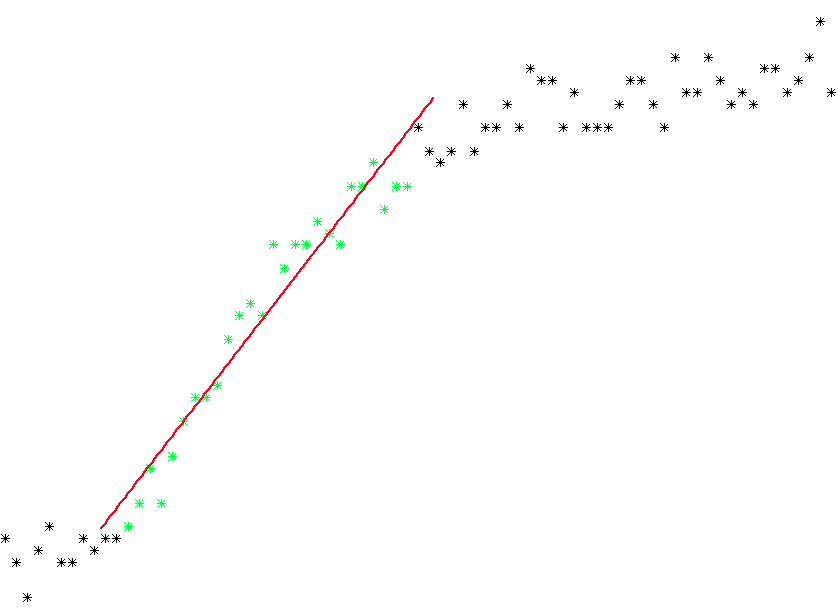
\includegraphics[scale=0.35]{./pictures/linFit}
 \caption{Linear fit of rising edge points (marked as green).}
 \label{linfit}
\end{figure}


\subsection{Results}
First data taking sequence ran about two weeks. Taken data were analysed by methods described in previous chapter and results are presented in the following graphs. The first two graphs describe 
optical power with respect to time (first from PM and second is the PMT pulse height).
\begin{figure}[H]
 \centering
 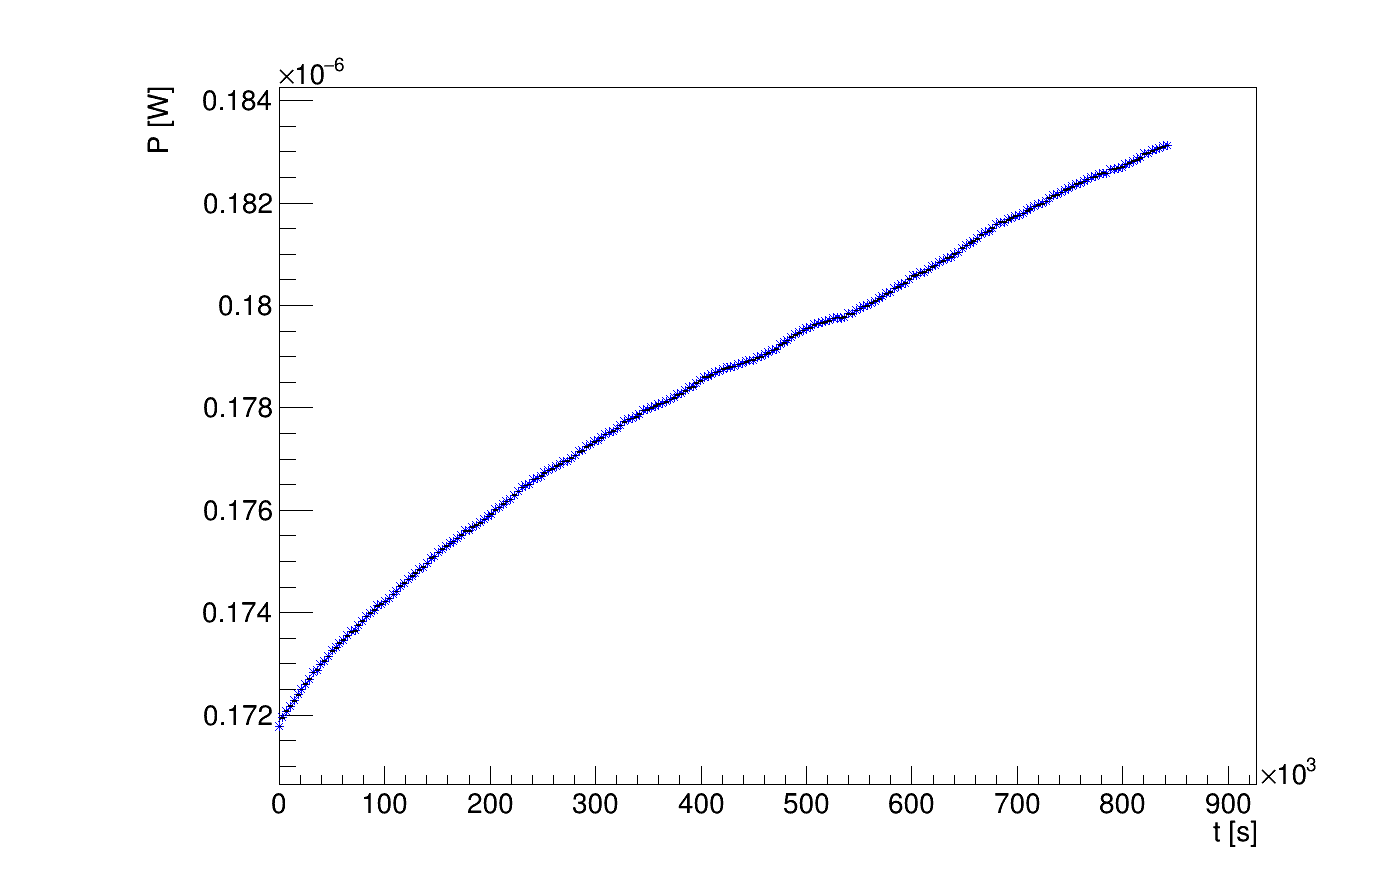
\includegraphics[scale=0.3]{./pictures/powers}
 \caption{Time evolution of optical power.}
 \label{pow1}
\end{figure}



\begin{figure}[H]
 \centering
 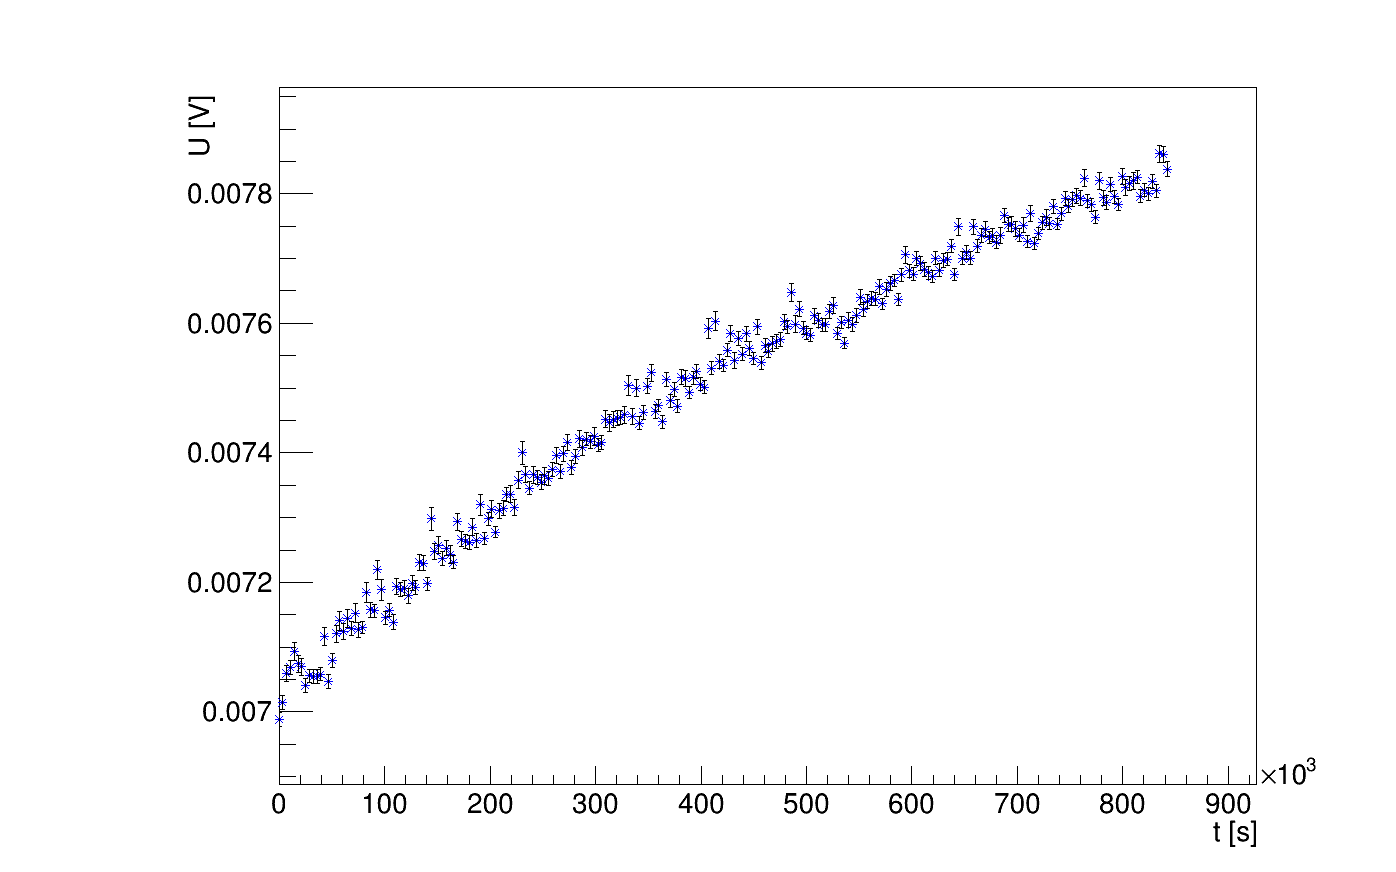
\includegraphics[scale=0.3]{./pictures/Height}
 \caption{Time evolution of the pulse's height.}
 \label{height1}
\end{figure}

In the next two graphs we present calculated heights and slopes.

\begin{figure}[H]
 \centering
 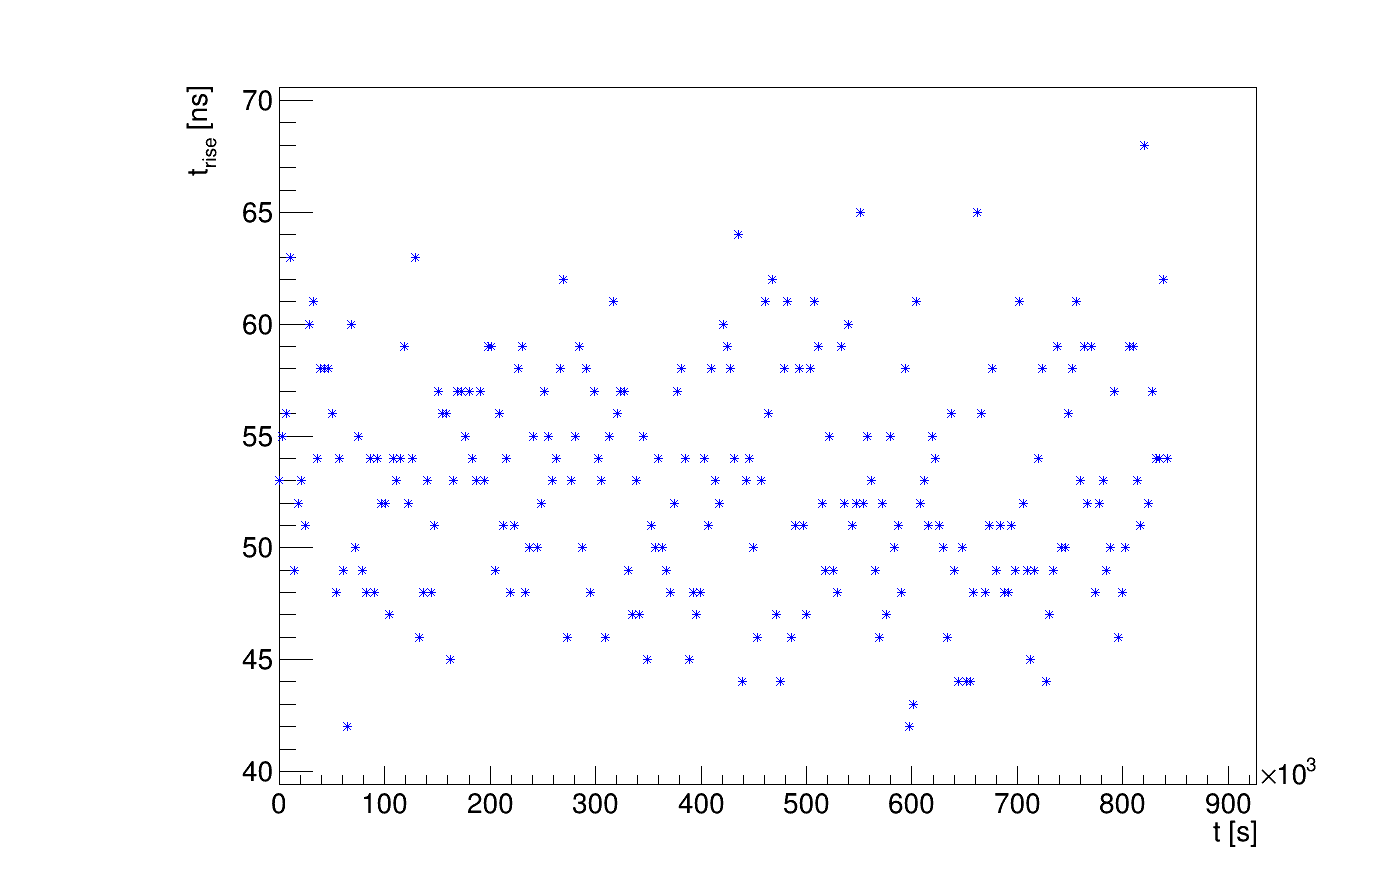
\includegraphics[scale=0.3]{./pictures/rise}
 \caption{Time evolution of the pulse's edge rise time.}
 \label{rise1}
\end{figure}

\begin{figure}[H]
 \centering
 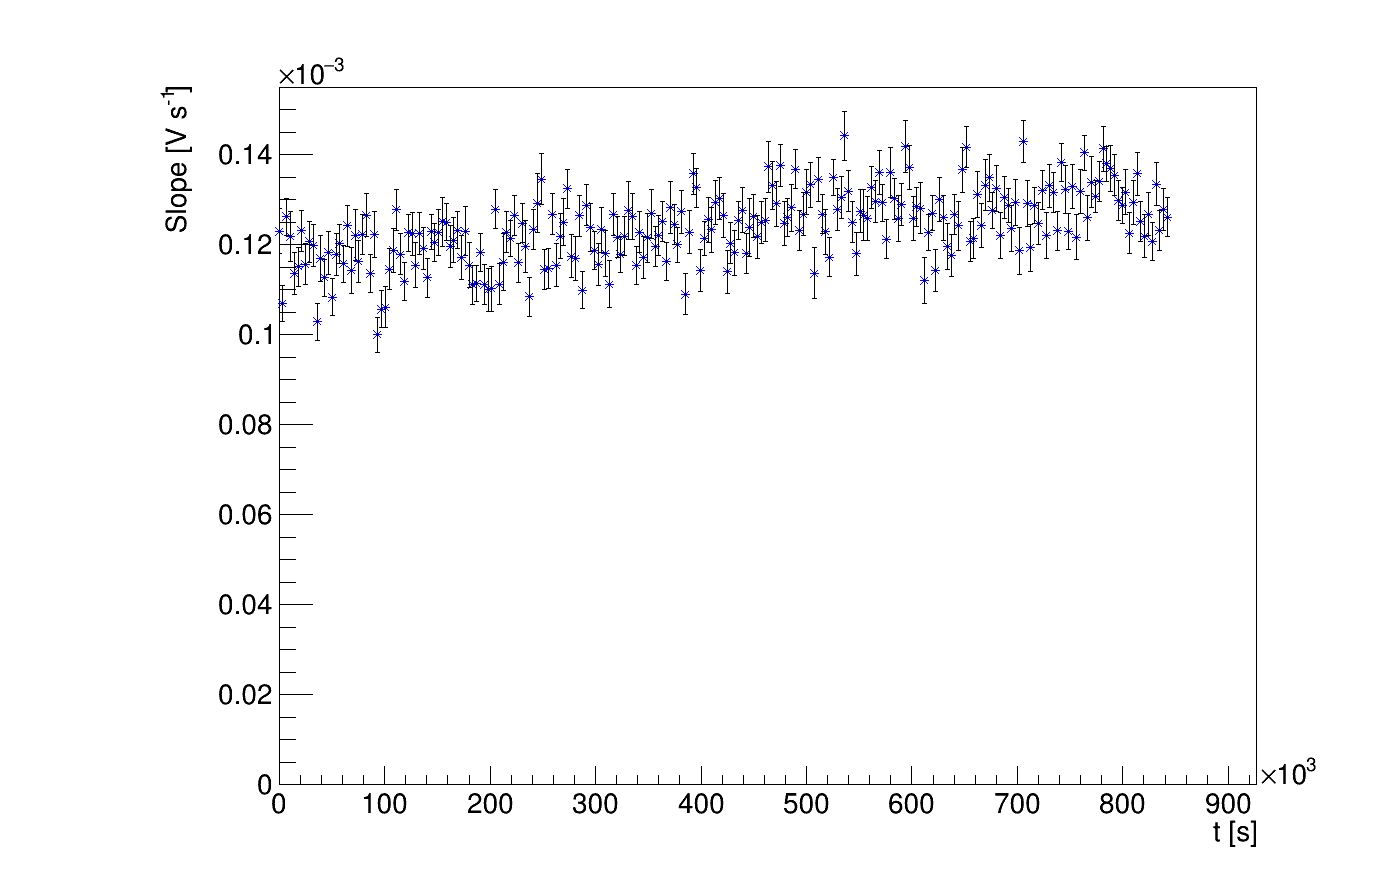
\includegraphics[scale=0.3]{./pictures/Slope}
 \caption{Time evolution of the pulse's edge slope.}
 \label{slope1}
\end{figure}

We also measured PMT's temperature for potential gain changes.
 
\begin{figure}[H]
 \centering
 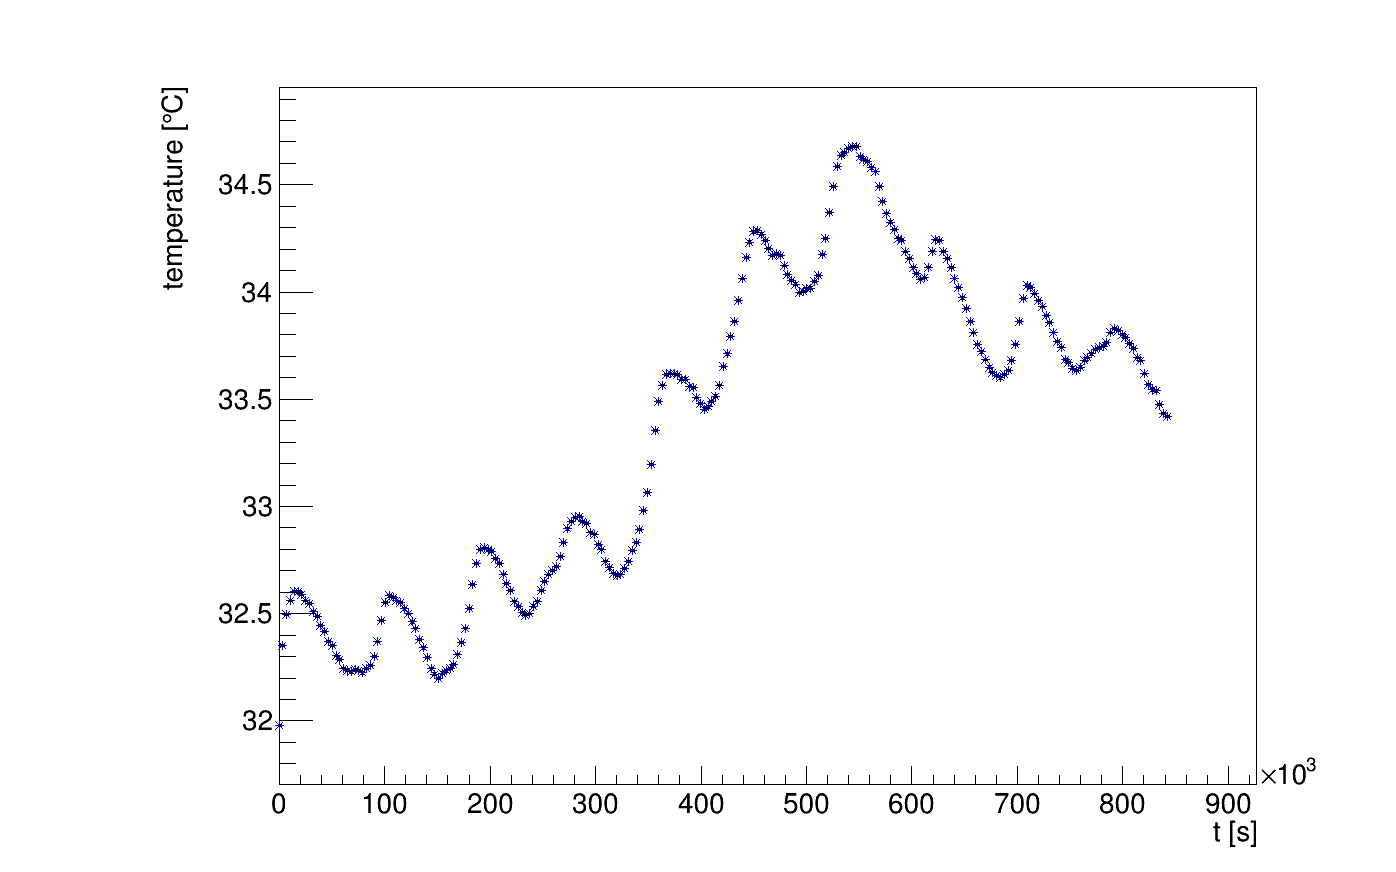
\includegraphics[scale=0.3]{./pictures/temperatures}
 \caption{Time evolution of the PMT's temperature.}
 \label{temp1}
\end{figure}

From analysed data we may observe that the power is rising over time. This fact is confirmed by two sensors - both PM and PMT. In case of PMT there may be the drift in gain over time. Gain drift may be caused by changes in voltage (equation \ref{gainVolt}) or in temperature. In case of temperature, the trend is not only rising as $U_{H}$'s trend does, so the $2_{\circ}$ change in temperature may play little role in $U_{H}$ increase, but it is not probably the main cause of this effect.
The graphs \ref{rise1} and \ref{slope1} shows that pulse is not deforming over time.
\par
The optical power instability may be caused by failures in LED driving circuit (changes in current flowing by diode) or by ageing processes in the UV diodes. The PM shows that the power increase is around $7 \%$ in 10 days, which is unacceptable for any calibration source. 
\par
To confirm this measured fact and check for possible causes of the optical power instability we repeated this measurement by few times with similar results. But during these measurements we used multimeter to monitor PMT's voltage. For measuring the current flowing by the diode in the internal current source circuit, we used the second channel of the osciloscope.

\begin{figure}[H]
 \centering
 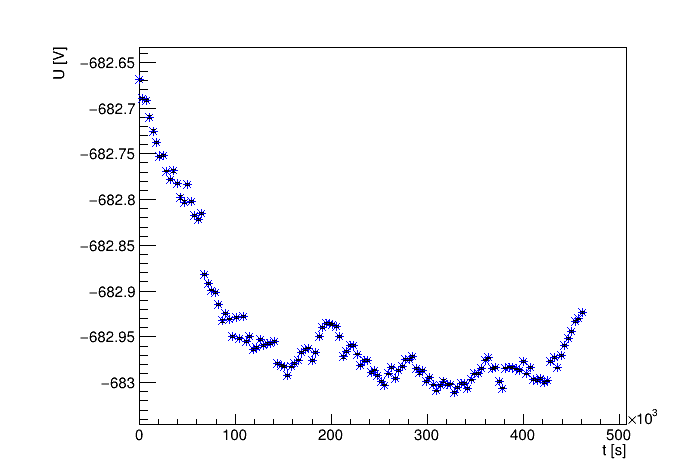
\includegraphics[scale=0.5]{./pictures/voltage}
 \caption{Time evolution of the PMT's voltage.}
 \label{PMTVolt}
\end{figure}

\begin{figure}[H]
 \centering
 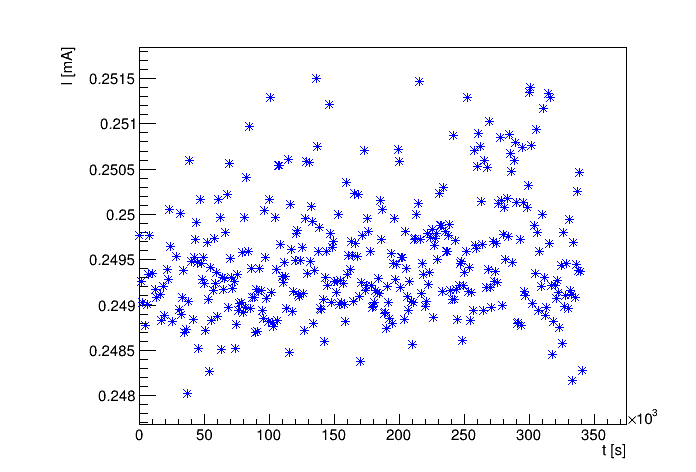
\includegraphics[scale=0.5]{./pictures/Current}
 \caption{Time evolution of the UV LED's current.}
 \label{LEDCurrent}
\end{figure}

Other measurements of optical power have ended in similar way. But by using the multimeter we can see that PMT's voltage is stable (fig. \ref{PMTVolt}). It is varying only about 0.4 V at the beginning.
\par
The measurement of current by oscilloscope was done and analysed in similar way as was done for the PMT's pulses. Both of them are PWM square pulses by shape. The oscilloscope's probe was connected to the 100$\Omega$ resistor, which is in serial to the LED and the current source and acted as a simple $U/I$ converter. As we can see in fig. \ref{LEDCurrent}, the current varies only a little over the value which was set ($I_\textrm{d} = 2.5$ mA), and thus the rising trend of optical power is definitely not caused by the current variations.


\section{UV LED diode ageing}
As was seen in results of previous measurements, the diode ageing process is the most probable cause of the changes in optical power. We tried to confirm this fact by ageing the similar UV LED (type MT3650W3-UV).
\par
The single UV LED powered by the current source lm334 on $I_\textrm{d} =$ 7.1 mA was mounted onto IS's port and the optical power in continual mode was measured by the PM16. For the additional correction - the $I_\textrm{d} $ was also measured by keysight multimeter.


\par
\begin{figure}[H]
 \centering
 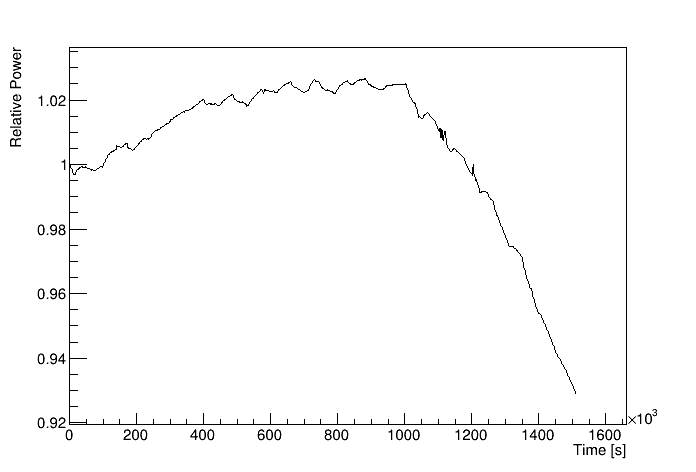
\includegraphics[scale=0.5]{./pictures/corrected1}
 \caption{Time evolution of the optical power of single UV LED.}
 \label{SingleDiod}
\end{figure}
\par
On the fig. \ref{SingleDiod} we can see that the optical power of single LED increased about $2 \%$ after one week. Then followed a stable interval which lasted about a week, but after that period the LED started "dying" and the power started to decrease.

\par
There are 2 major possibilities to fix the LED power variation problem. The first possibility is to monitor the time usage of the UV source the and according to that recalibrate the source, but the behaviour may vary diode from diode and thus it has many disadvantages. The second and more accurate approach is to regulate the power by an optical feedback.    


%------------------------------------------------
\section{Optical feedback - potential fix}
% -----------------------------------------------
One way to handle the ageing process of UV LED diodes is to monitor the power and according to the changes set the diode current $I_\textrm{d}$. To achieve that, we tried to develop a prototype of optical feedback concept, which is based on detection UV photodiode. 
\par
The part of optical power is reflected from LED to photodiode. Photocurrent induced this way is converted to voltage which is read by ADC (analog-digital converter). This information is then used by the STM32 board to adjust the current level by DAC. One problem is that the optical power is delivered in pulses, and thus it is necessary to sample these pulses and determine the height.
\par
\subsection{Detection photodiode}
As detection photodiode which we chose is GUVV-T10GD. It is guaranteed to be UV-A sensor with wavelength responsivity from 230 to 395 nm. However, it is necessary to test more of its properties, because some of the properties, which are essential for our application, are not shown in datasheets and probably haven't been yet measured - temperature dependency of the dark current, responsivity to 10 $\mu$s square signals and ageing processes. The reverse voltage of photodiode $U_\textrm{r}$ could go up to 2 V. With higher the $U_\textrm{r}$ is, the lower is the diode's capacity.
\par
\subsubsection{Dark current}
Information of dark current is very important. We need to know if the signal levels are much greater than dark current. We measured dark current with 7 set temperatures. Current was measured by Keithley 2470 picoammeter. Temperature was set by autoregulated transistor heating plate. The transistor plate is driven by STM32 nucleo's DAC. The nucleo is controlled by the RPi. The RPi also communicates with picoammeter and controls the entire data acquisition. We measured two series - one with reverse voltage $U_\textrm{r} = 0.1$ V and second with reverse voltage $U_\textrm{r} = 1$ V. The picoammeter is also capable of adjusting voltage, so it was used as a source of reverse voltage.

\begin{figure}[H]
 \centering
 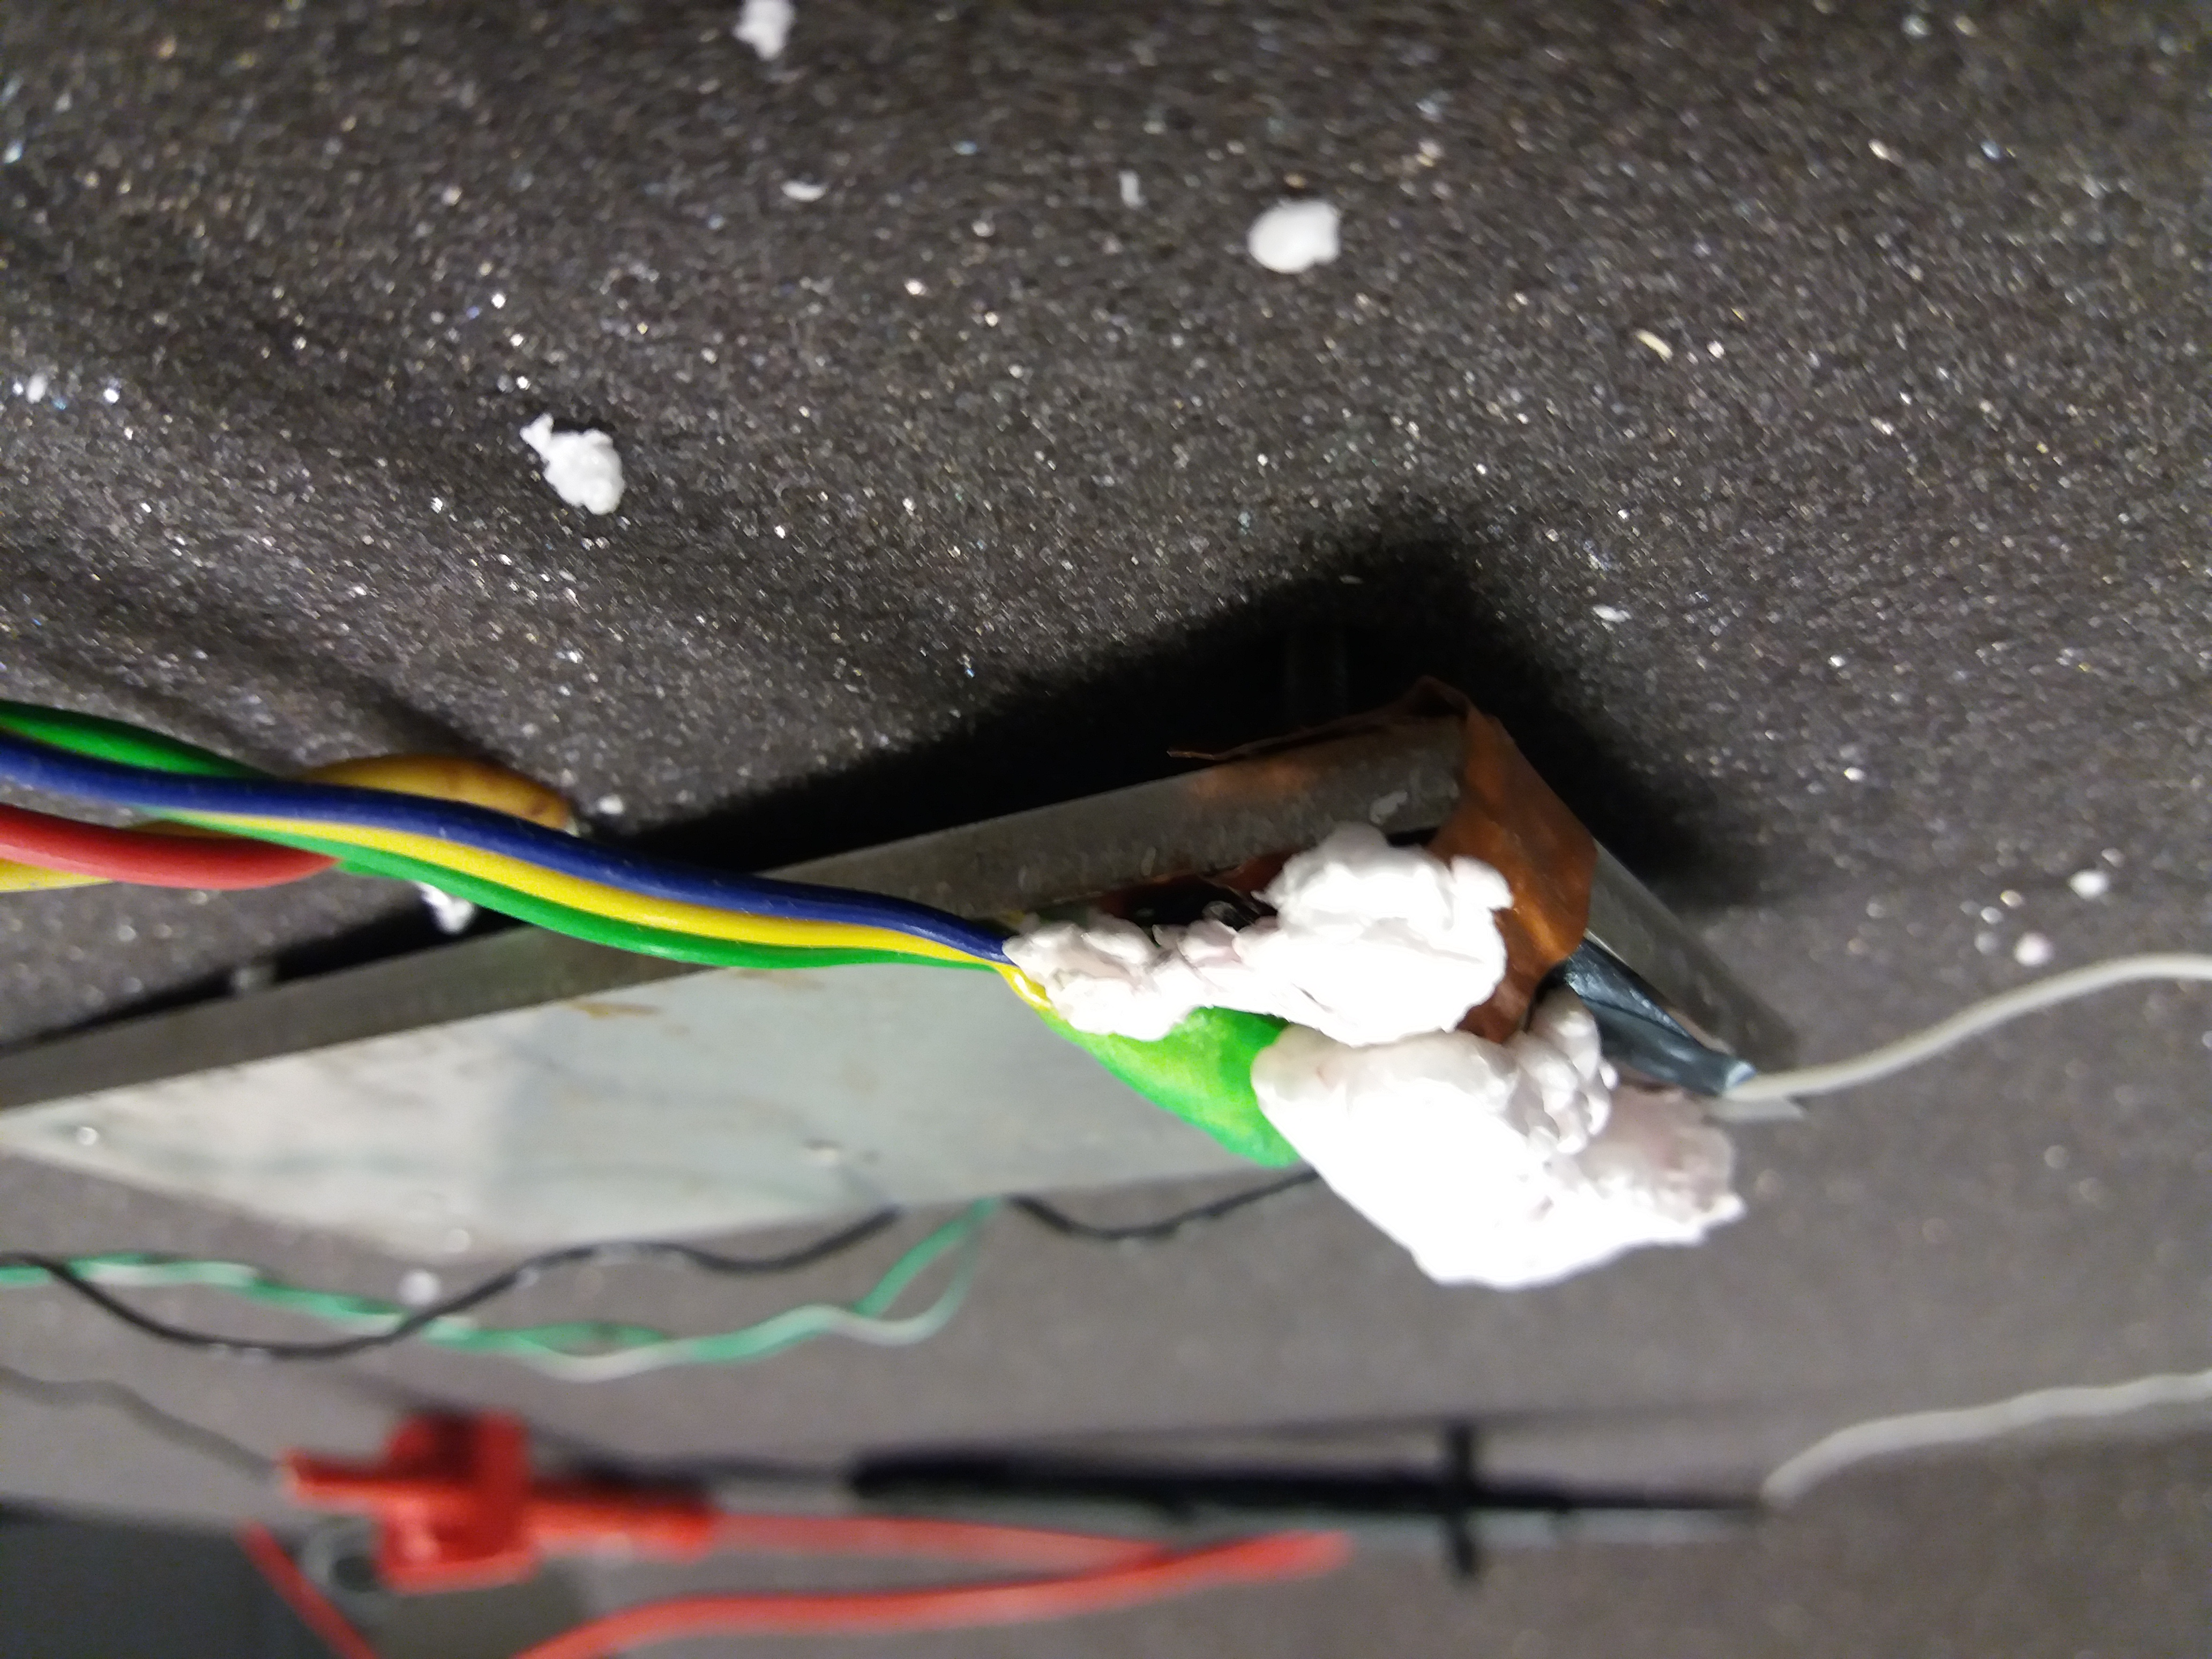
\includegraphics[scale=0.09, angle = 180]{./pictures/DiodeHeat}
 \caption{UV detection diode mounted on heating plate, covered by insulating material. The thermometer is mounted next to it.}
 \label{heatDiode}
\end{figure}


\begin{figure}[H]
 \centering
 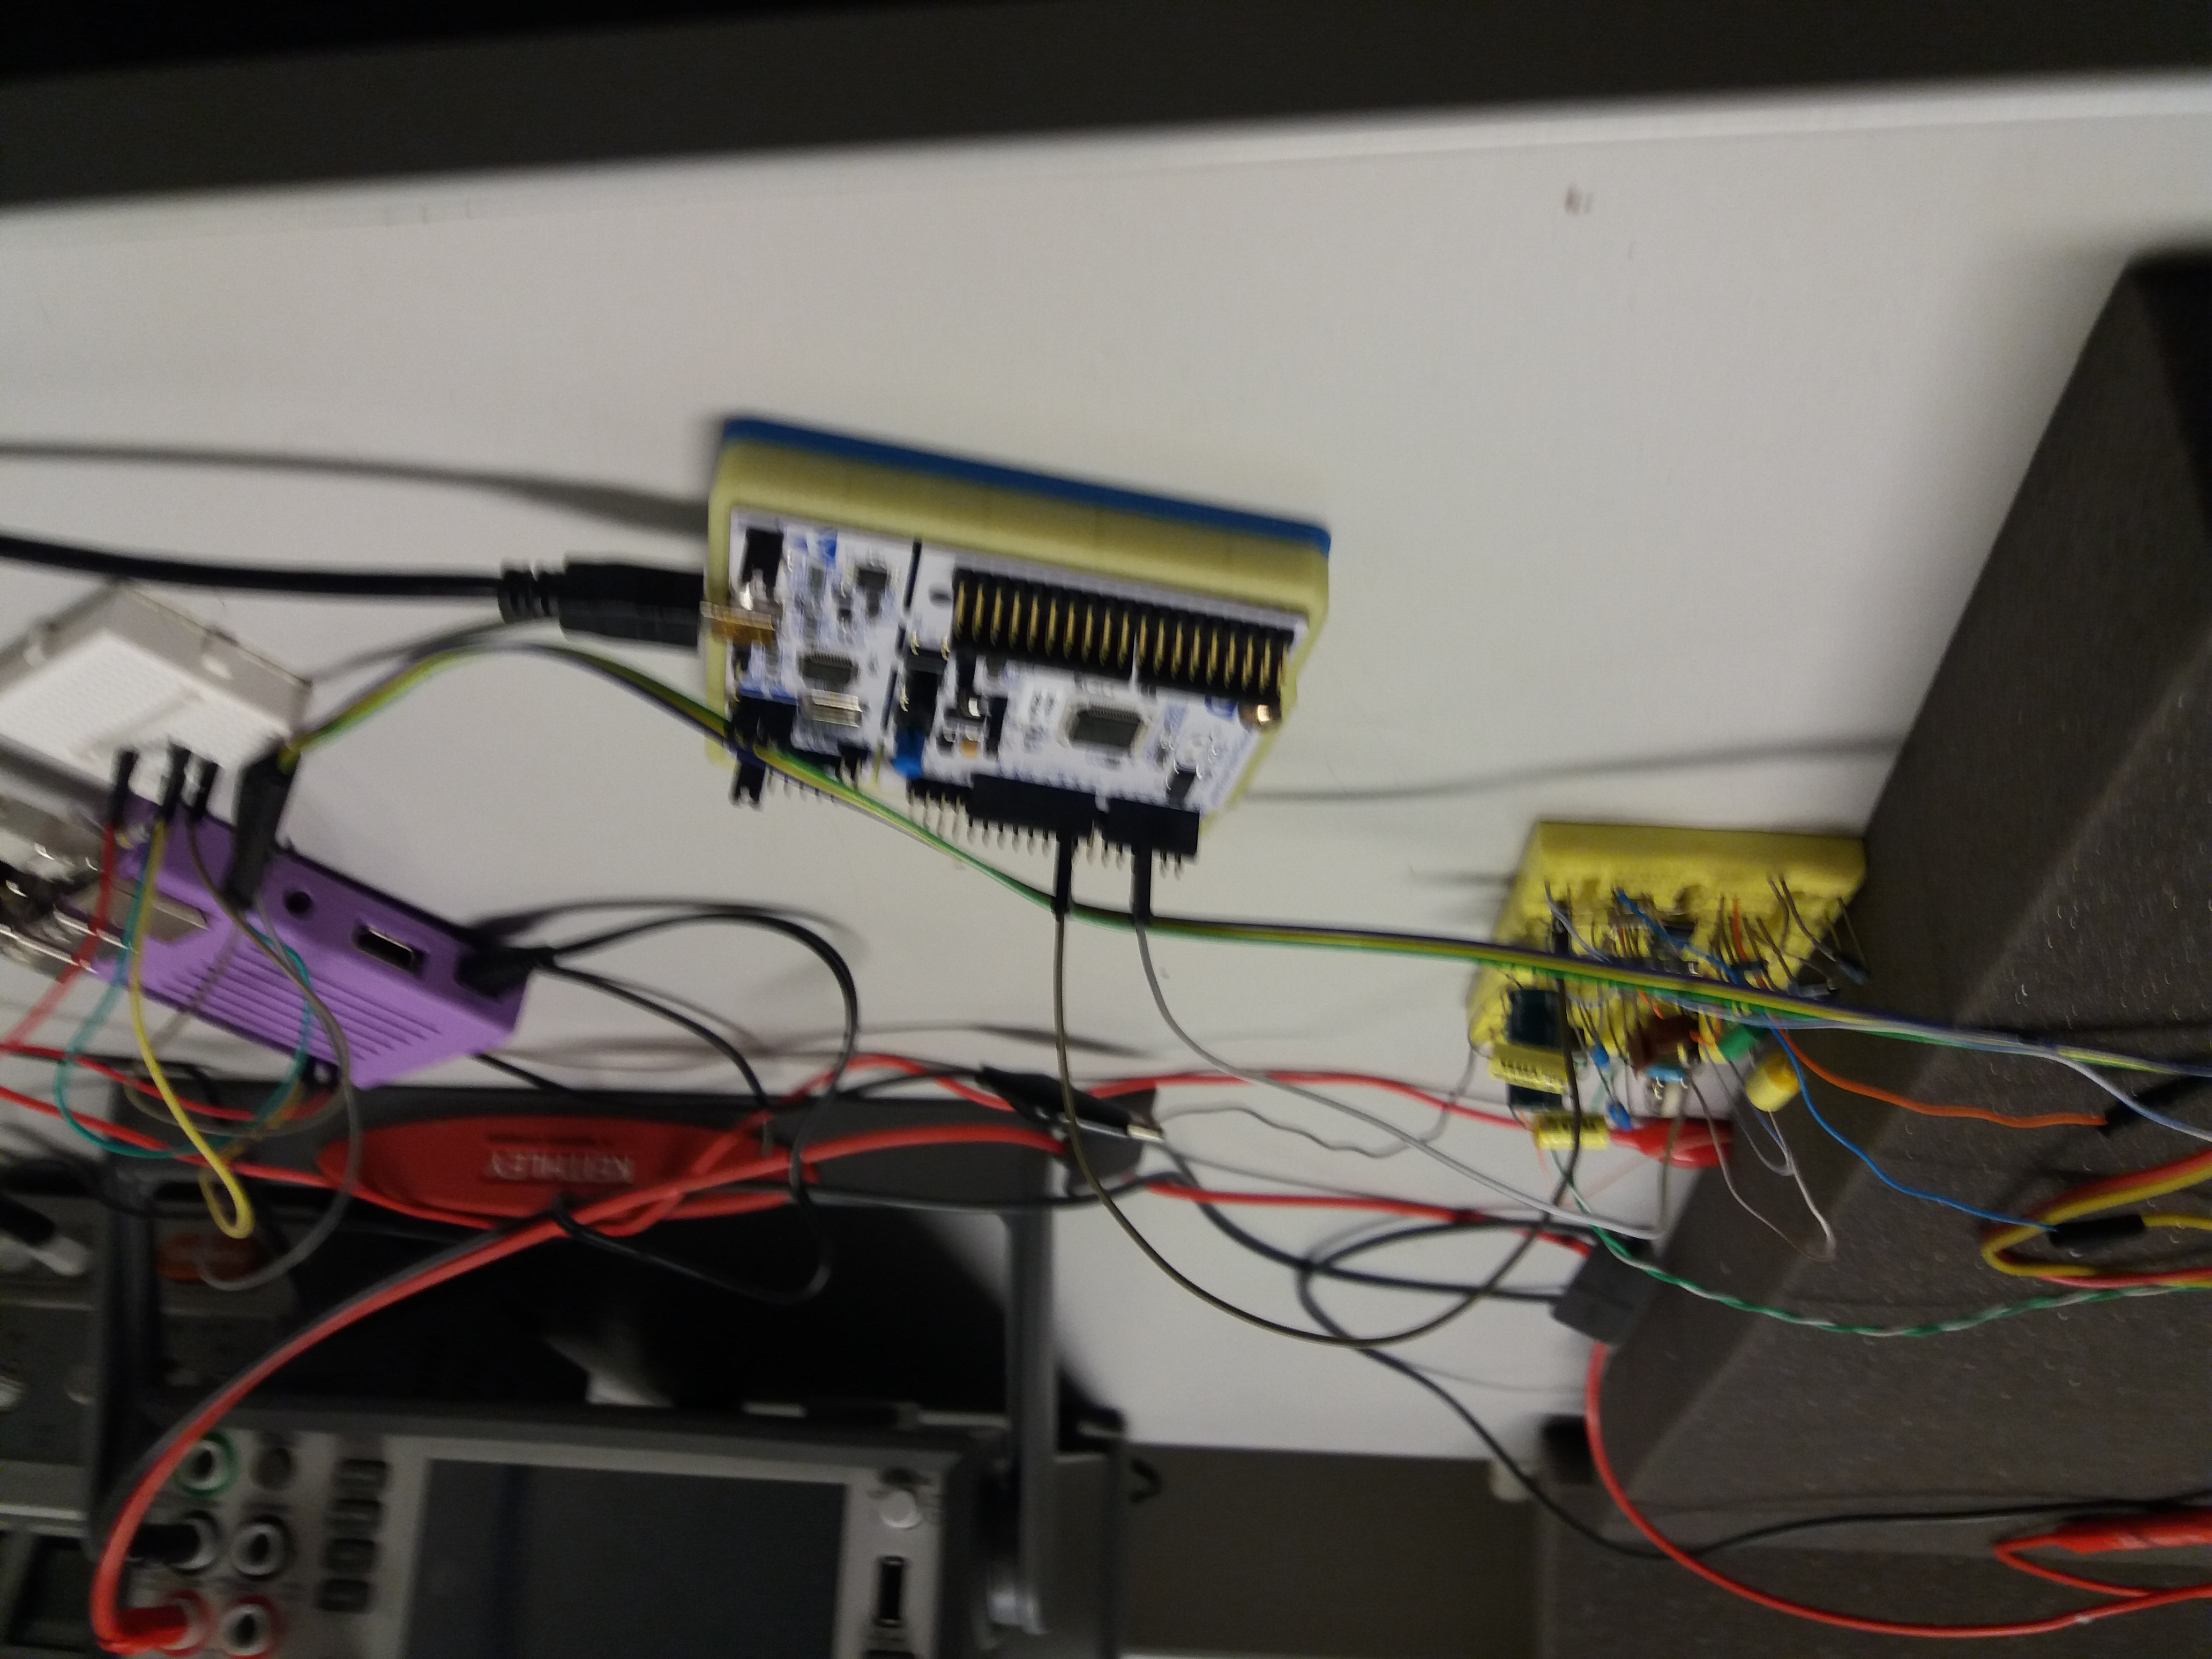
\includegraphics[scale=0.09, angle = 180]{./pictures/heating}
 \caption{Heating control and measurement control. From the left - heating circuit, STM32 nucleo, RPi}
 \label{heating}
\end{figure}



\begin{figure}[H]
 \centering
 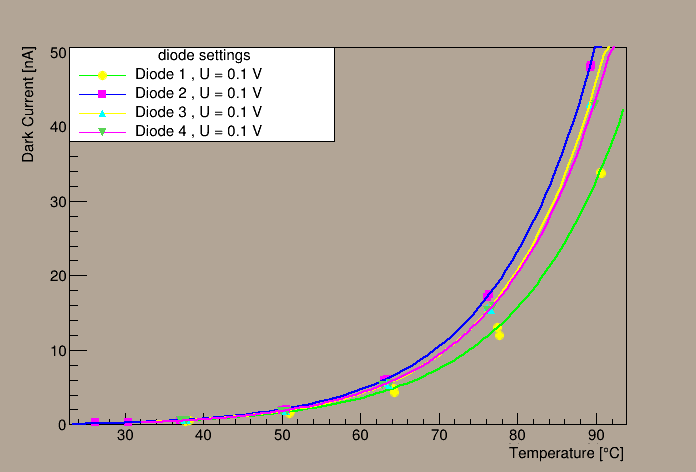
\includegraphics[scale=0.5]{./pictures/01V}
 \caption{Dark currents with the reverse voltage $U_\textrm{r}= 0.1$ V.}
 \label{01V}
\end{figure}

\begin{figure}[H]
 \centering
 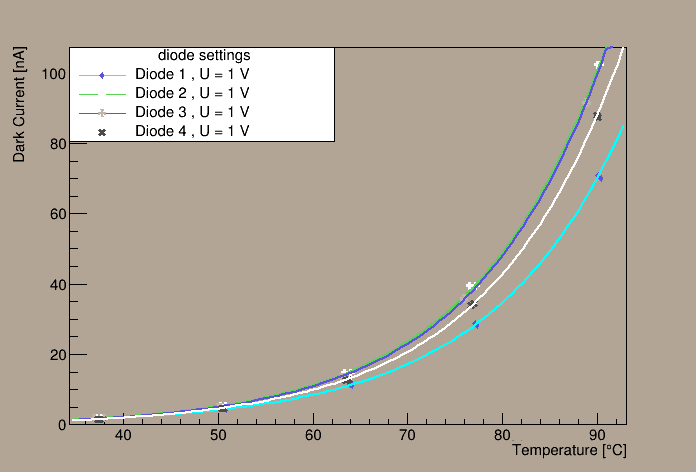
\includegraphics[scale=0.5]{./pictures/1V}
 \caption{Dark currents with the reverse voltage $U_\textrm{r}= 1$ V.}
 \label{1V}
\end{figure}


We measured 5 diodes. However, the dark currents of one diode were on abnormal level, and that's why its characteristics are not plot in graphs with others. This diode was not suitable for our application.
\par

From the measured data we can see, that for the expected operating temperatures ($t < 50^{\circ}C$), the dark current is $I_{dark} < 10$ nA. 

\subsubsection{Signal responsivity}
By direct illumination of the photodiode by the UV LED ($I_d = 7.5 $ mA) we are able to induce photocurrent about $I_\textrm{p} = 5$ $\mu$A, which is of the higher order than the measured dark current.
\par
To test responsibility of the square pulses, we integrated the photodiode into the $I/U$ trans-impedance amplifier with the op-amp ADA4805 with feedback parameters $R_\textrm{F} = 100$ k$\Omega$ and $C = 9$ pF. We illuminated the photodiode by the UV LED connected to the square pulse generator. The response could be seen on fig. \ref{response}.

\begin{figure}[H]
 \centering
 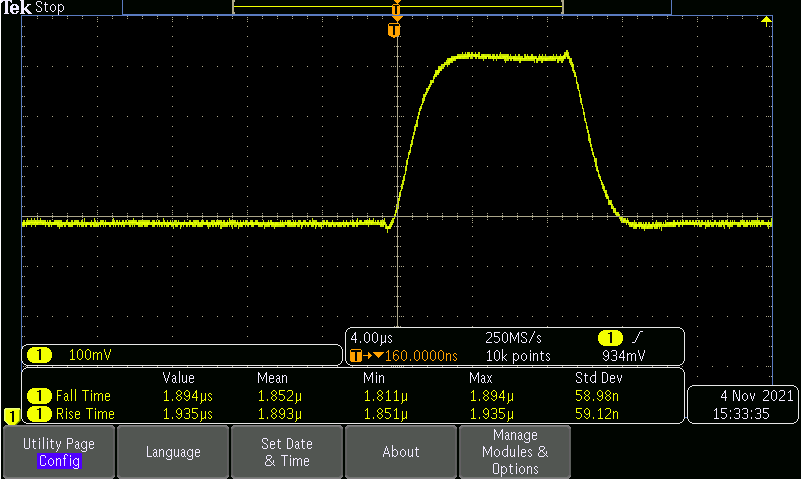
\includegraphics[scale=0.5]{./pictures/pulse}
 \caption{Photodiode's response on 10 $\mu$s square pulse.}
 \label{response}
\end{figure}


This way we are able to see the pulsing UV LED light. However, the rising edge of feedback pulse is deformed. 

\subsubsection{Artificial ageing}
For the feedback photodiode, the time stability is very important. It has to last much more than the LED. To test the long-time stability, we tried to artificially age the feedback photodiode. It is well-known fact from the molecular physics, that the diffusion coefficients of most materials depends on temperature and they grow with increasing temperature. So we tried to speed up the ageing by holding the photodiode under the maximum of operating temperature (on $80^{\circ}$C) for one week. During that period, the photodiode was illuminated by UV LED and the photocurrent was measured (fig. \ref{agingPhotoCurrent}).


\begin{figure}[H]
 \centering
 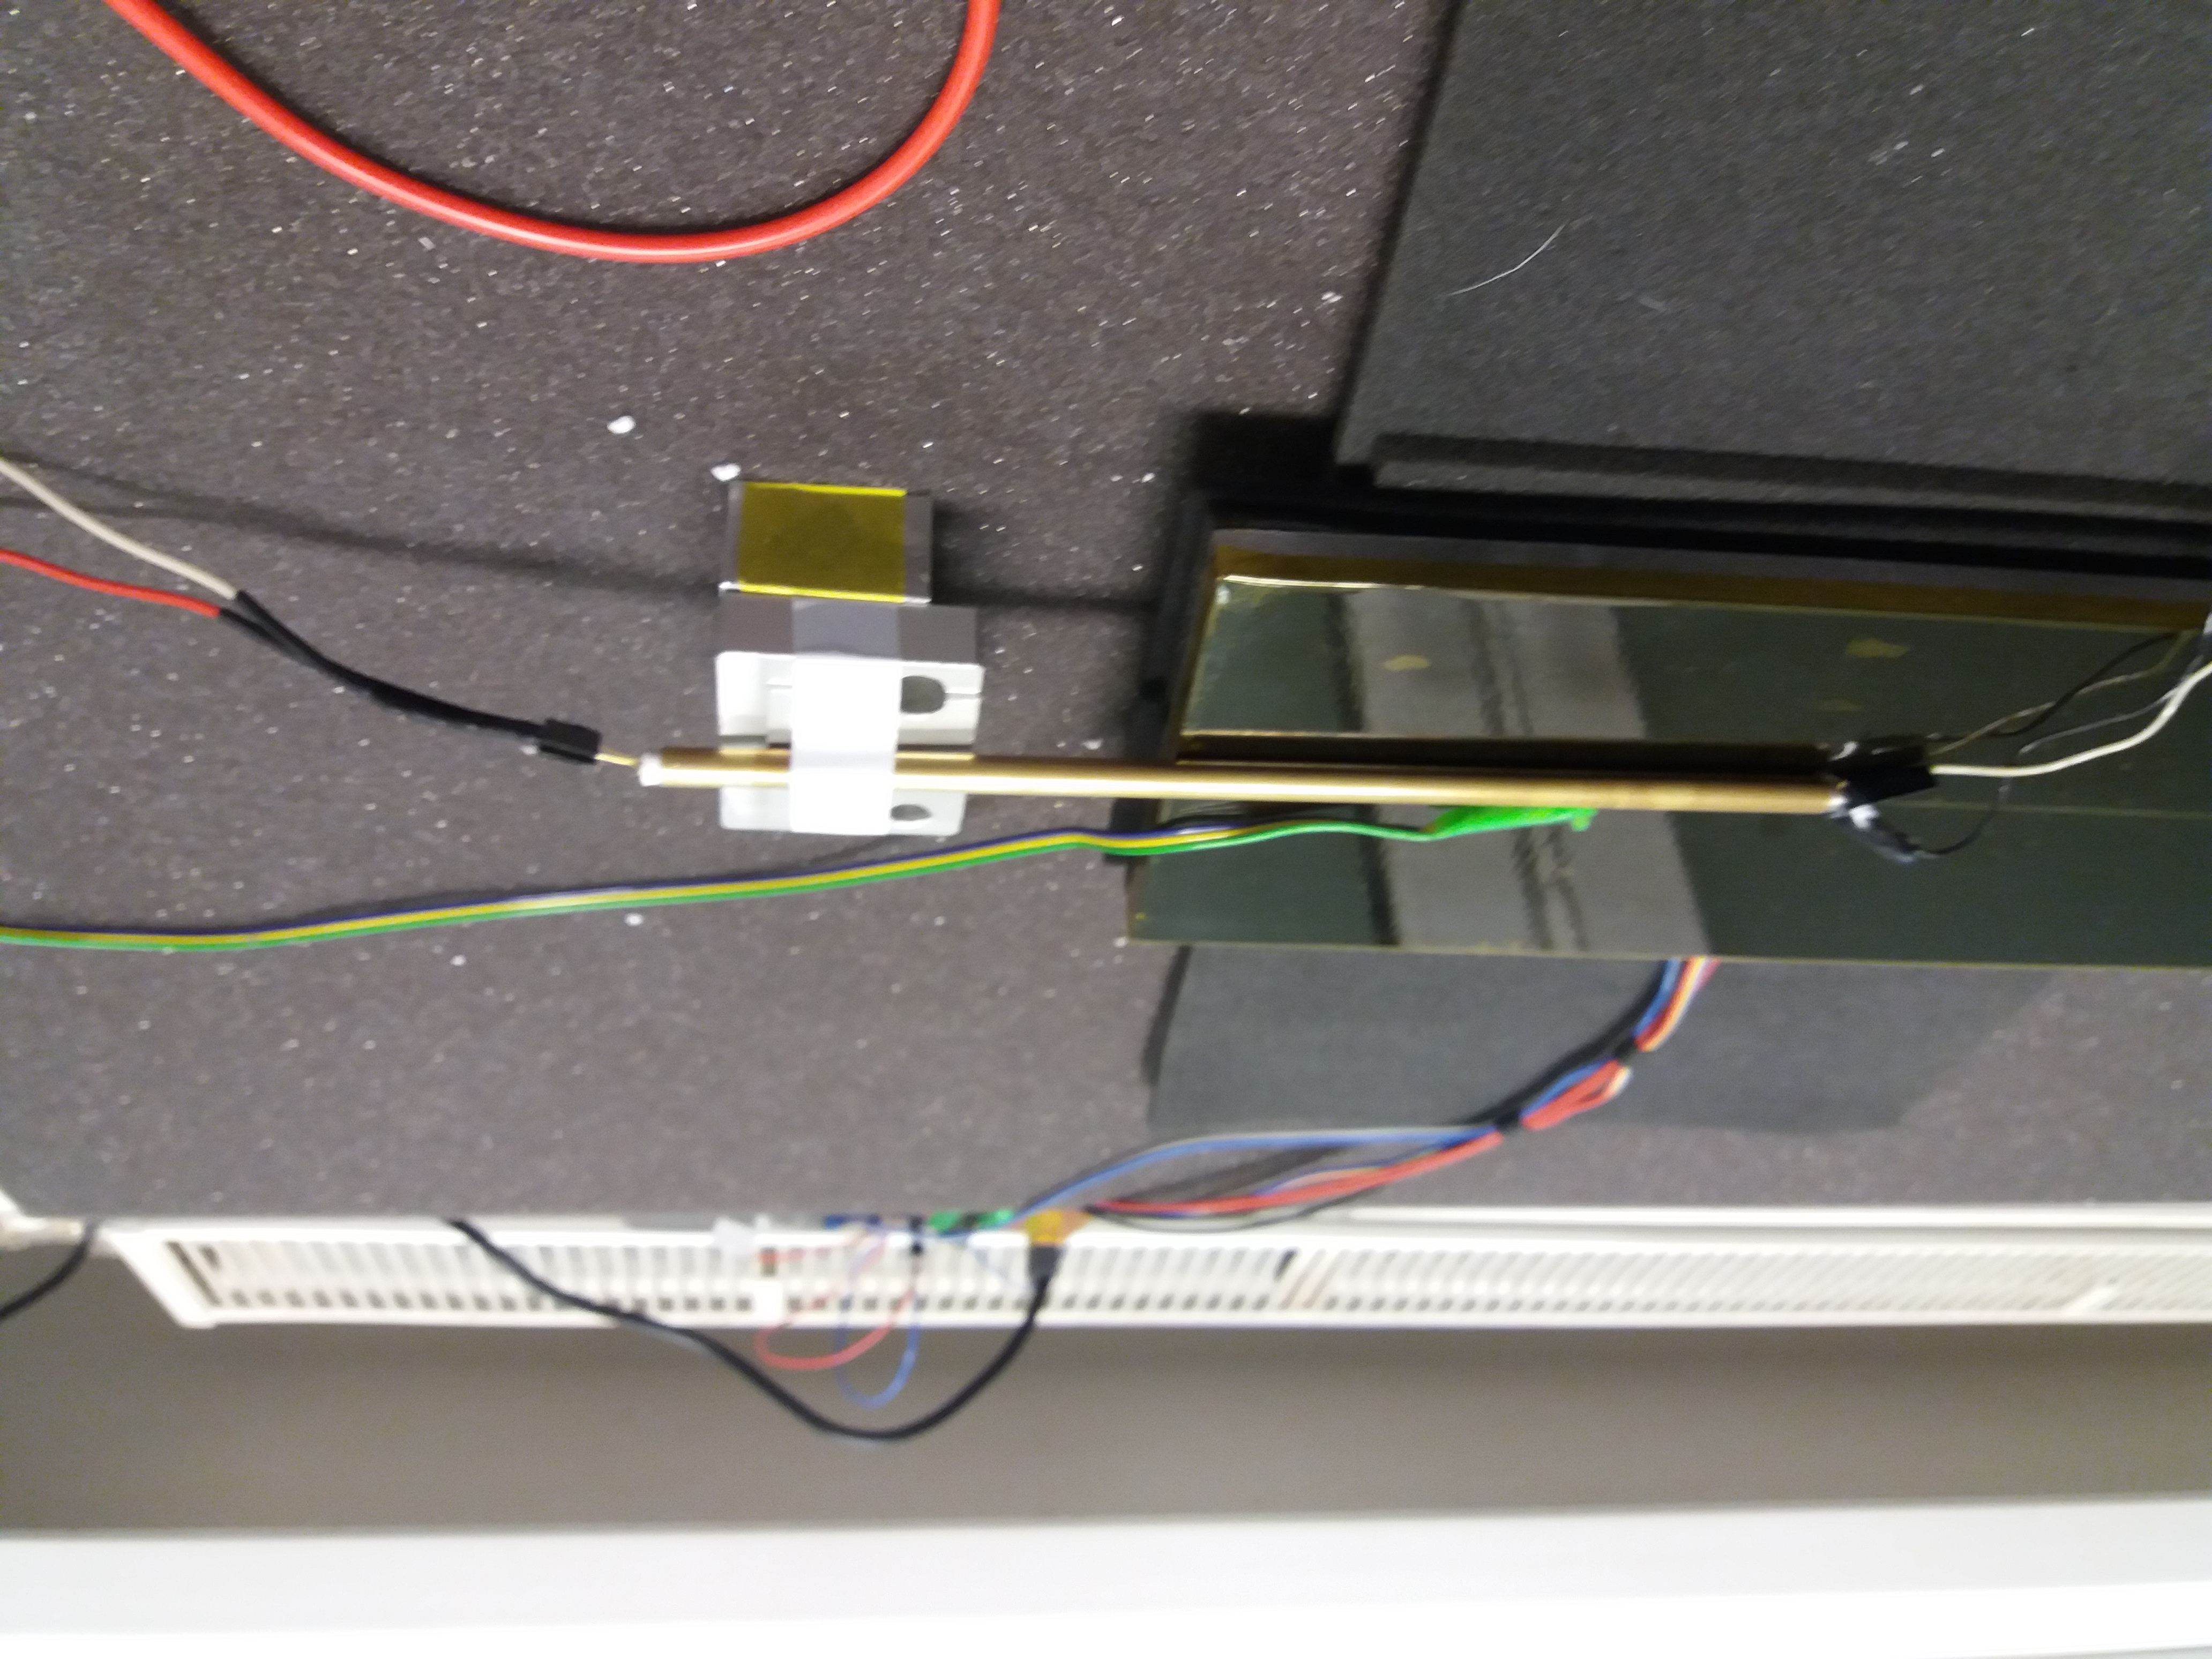
\includegraphics[scale=0.08, angle=180]{./pictures/TempDestrc}
 \caption{Photodiode mounted on bigger transistor heating and illuminated by LED through pipe.}
 \label{aging}
\end{figure}


\begin{figure}[H]
 \centering
 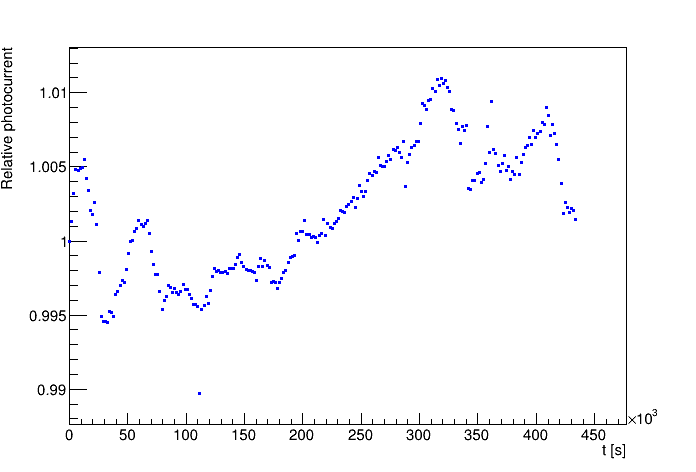
\includegraphics[scale=0.5]{./pictures/ArtiAging}
 \caption{Time evolution of the photodiode's photocurrent.}
 \label{agingPhotoCurrent}
\end{figure}

The time evolution shows that the photodiode's photocurrent increased around 1 $\%$ over one week. However, this small variation is probably caused by the LED ageing, as was shown before. 
\par
Due to the fact, that any bigger drift in sensitivity was not observed under the bad conditions, we come to a conclusion that the feedback photodiode is much more stable than the LED.

\subsection{Feedback concept and testing}

The original concept circuit was modified by adding the feedback part, which consists of two op amps - primary acts as transimpedance amplifier to convert induced photocurrent into the signal voltage and the secondary acts as a simple voltage amplifier. The additional scheme can be seen on fig. \ref{Amplifier}.
   
\begin{figure}[H]
 \centering
 
\includegraphics[scale=0.5]{up_logo_bw}
 \caption{2 - Amplifier with photodiode scheme.}
 \label{Amplifier}
\end{figure}

The UV LED is mounted in position to deliver power into the photodiode and also to an output port. The optomechanical system can be seen on fig. \ref{Optomechanics}.

\begin{figure}[H]
 \centering
 
\includegraphics[scale=0.5]{up_logo_bw}
 \caption{Optomechanics of prototype.}
 \label{Optomechanics}
\end{figure}


However, the UV source is designed to deliver 10 $\mu$s pulses, so, to determine the signal level, it is necessary to sample this pulse. 

\subsubsection{Sampling}

To perform the pulse sampling, the hardware with enough capabilities has to be used. STM32 board Nucleo F446RE offers various timers (for PWM generation and advanced triggering), both 12-bit ADC and DAC (digital to analog converter) and a DMA (direct memory access) feature. The ADC combined with DMA can flush the sampled data directly into the memory and may exceed the sample rate over 1 MS/s.

\par

The other problem is the time synchronization of sampling with the pulse, to achieve that  . The sampling procedure can be seen captured by oscilloscope on fig. \ref{procedure}.



\begin{figure}[H]
 \centering
 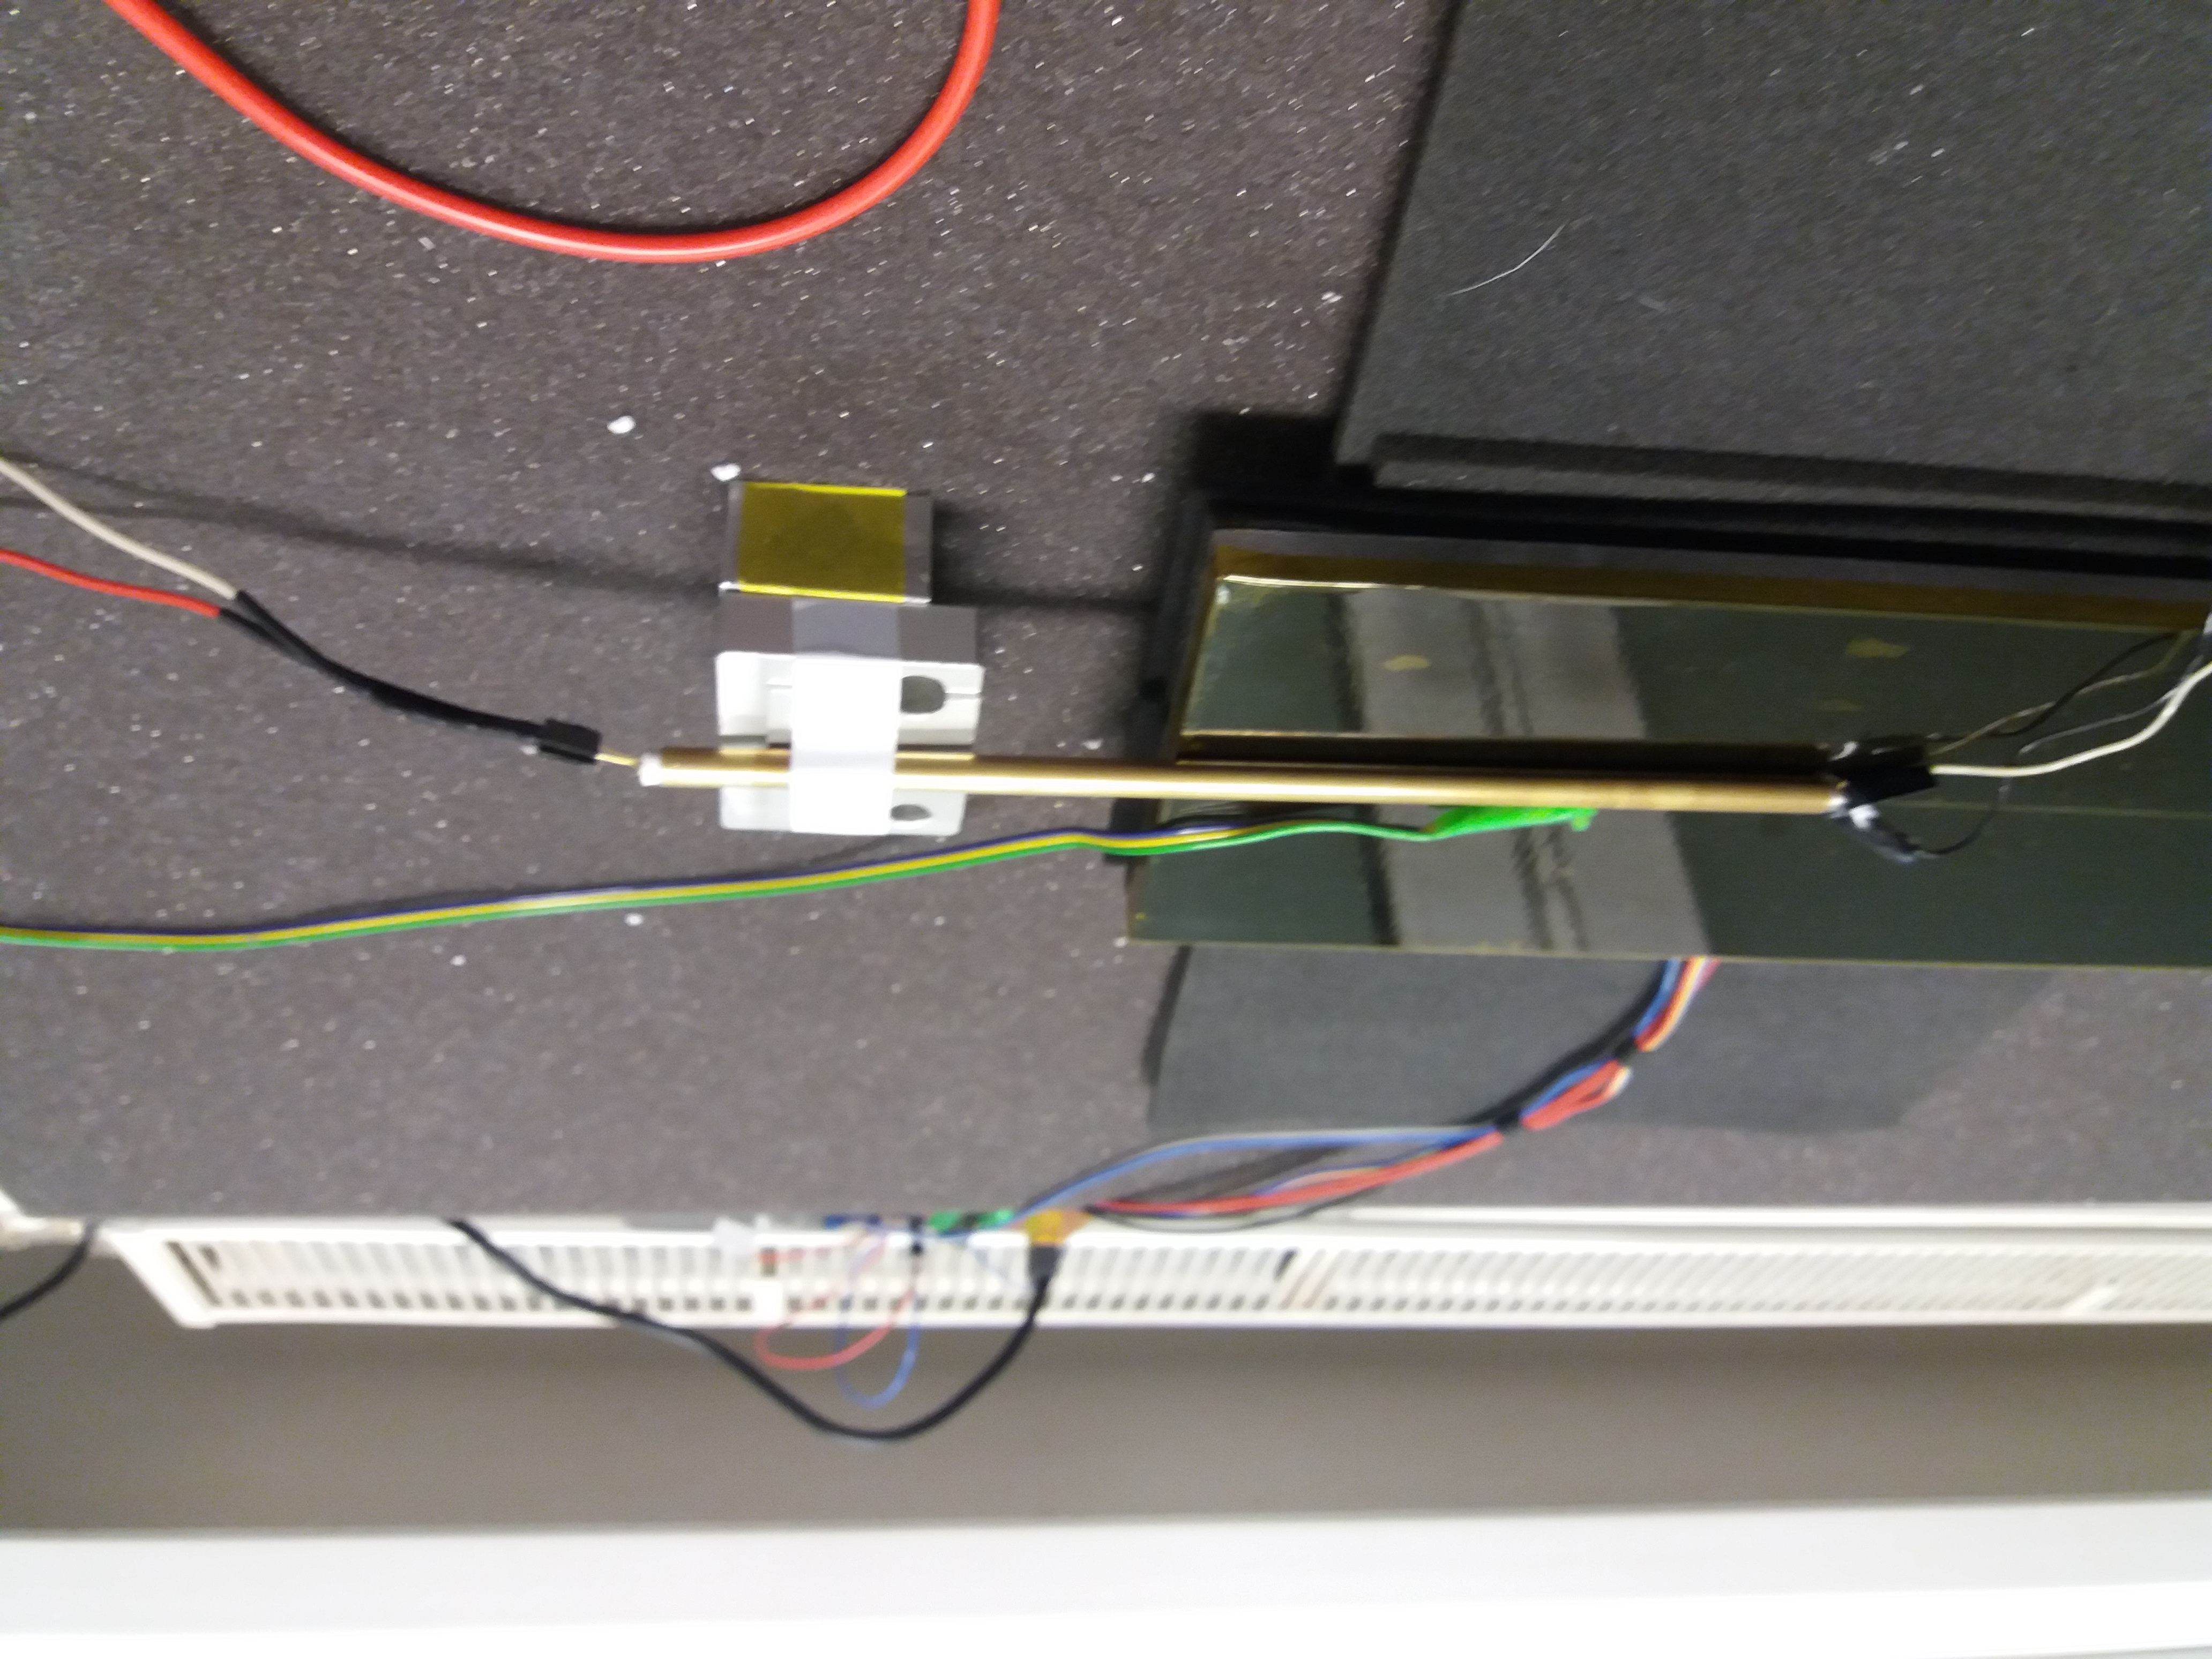
\includegraphics[scale=0.08, angle=180]{./pictures/TempDestrc}
 \caption{Photodiode mounted on bigger transistor heating and illuminated by LED through pipe.}
 \label{procedure}
\end{figure}



\par

The ADC and DAC reference is 3.3 V made from the supply voltage stabilizer, which does not have the required accuracy and may vary with the supply voltage. For the feedback purposes the STM32 reference pin was reconnected to the external, more accurate 2 V reference along with a 50nF capacitor to prevent board's internal oscillators from jamming the reference stability.     




\subsubsection{Sampling}


\subsubsection{Longtime testing}

%------------------------------------------------
% -----------------------------------------------



% -----------------------------------------------
% %%%%%%%%%%%%%%%%%%%%%%%% End of file %%%%%%%%%%%%%%%%%%%%%%%%
